\documentclass[oneside,a4paper,12pt]{memoir}
\usepackage{amssymb,amsmath}
\usepackage{chngcntr}
\usepackage{color}
\usepackage[latin1]{inputenc}
\usepackage[ruled,vlined,linesnumbered]{algorithm2e}
\usepackage{graphicx}
%\usepackage{caption}
\usepackage{subcaption}
\usepackage{url,hyperref}
\usepackage{booktabs}
\usepackage{float}
\usepackage{colortbl}
\usepackage{comment}
\usepackage{ulem}
\usepackage{todonotes}
\usepackage{listings}

\begin{document}
\title{SAIM - Manual}
\author{Klaus Lyko}                                                  
\maketitle

\newpage
\tableofcontents*
\chapter{Introduction}
Links between instance are of central importance for the Semantic Web and for a large number of tasks, such as data integration, federated querying and knowledge retrieval. Finding those links is the subject of Link Discovery (LD).
Two main problems arise when trying to discover links between data sets.

First, naive solutions have to compare all instances of a source knowledge base with all instances of the target knowledge base, thus having a quadratic time complexity. Second, one have to guarantee the quality of those links. 
To address the first problem time efficient algorithms and frameworks such as SILK\footnote{\url{https://www.assembla.com/spaces/silk/}} and LIMES\cite{NGAU11} have been developed to reduce the number of comparisons. For the second problem both supervised (e.g. \cite{NGLY12, NGO+13}) and unsupervised ({e.g. \cite{NIK+12}}) machine learning approaches have been developed.

SAIM \footnote{SAIM stands for (\uline{S}emi-)\uline{A}utomatic \uline{I}nstance \uline{M}atcher.}  encompasses solutions for both problems within one interface. It is based upon algorithms implemented in the LIMES\footnote{\url{http://limes.sf.net/}} framework which have been shown to outperform state-of-the-art in previous work w.r.t. time-complexity \cite{NGON12c}. SAIM offers an intuitive GUI for experts to manually create Link Specifications while implementing the supervised and unsupervised machine learning algorithms EAGLE \cite{NGLY12}	and COALA \cite{NGO+13} respectively, which have been shown to lead to highly accurate link specifications.

This manual will cover the complete workflow of SAIM. Starting in chapter \ref{kbdefinition} from scratch it will cover the process of defining the endpoints(\ref{endpoint}), class restrictions(\ref{classes}) and properties(\ref{properties}) of the knowledge bases to link. Chapter \ref{manual} describes how experts can build link specifications manually. Chapter \ref{selfconfig} and \ref{learning} discusses the unsupervised and supervised learning algorithms respectively. Finally, chapter \ref{features} covers additional features of SAIM such as saving and loading link specifications, uploading RDF dumps.

%%%%%%%%%%%%%%%%%                                  ENDPOINTS 													%%%%%%%%%%%%%%%%%%%%%%%%%
\chapter{Source and Target Endpoint definition}
\label{kbdefinition}
	Figure \ref{fig:MainWindow} shows SAIM upon startup.
	\begin{figure}
		\centering
		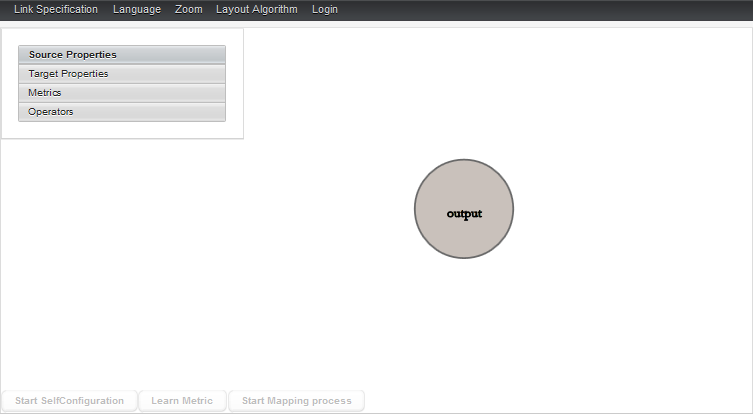
\includegraphics[width=0.8\textwidth]{images/main.png}
		\caption{The main window of SAIM is divided into three parts: A \emph{menu bar} at the top, an \emph{accordion} panel to the left and the \emph{metric panel} at the center.}
		\label{fig:MainWindow}
	\end{figure}
	As all no link specification is defined yet the 3 buttons at the bottom are deactivated and the accordion panel is empty. To start a Link Specification we go to the menu \texttt{Link Specification}. Figure \ref{fig:menu_start} shows the available menu entries:	
	\begin{enumerate}
		\item \texttt{Start new configuration} Start a new Link Specification from scratch.
		\item \texttt{Import Link Specification} To Import Link Specifications. It is covered in section \ref{ImportExport}.
		\item \texttt{Export Link Specification} Let you save Link Specifications on you local machine. It is covered in section \ref{ImportExport}.
		\item \texttt{Info} Will open a window with basic information about us.
	\end{enumerate}
	\begin{figure}
		\centering
		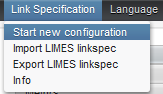
\includegraphics{images/menu_start.png}
		\caption{The \texttt{Link specification} menu.}
		\label{fig:menu_start}
	\end{figure}
	
	\section{Endpoints}
	\label{endpoint}
	To start a link specification we have to specify the RDF data sources dubbed \textit{Source} and \textit{Target Endpoint}. To do so go in the menu bar to \texttt{Link Specification} $>>$ \texttt{Start new configuration} as depicted in figure \ref{fig:menu_start}. This will open a Window as shown in figure \ref{fig:endpoint}. \\
	There are fields to be set:
	\begin{enumerate}
		\item \texttt{Endpoint URL} The URL of the public accessible SPARQL endpoint.
		\item \texttt{ID/Namespace} identifies the endpoint. Should be a string differentiating the endpoint as this entry is used be certain class matchers later.
		\item \texttt{Graph} (optinal) URI of a specify RDF graph.
		\item \texttt{Page Size} (optional) for pagination of SPARQL queries.
	\end{enumerate}
	It is possible to use predefined Presets from a list, such as DBPedia as depicted in the top layer of figure \ref{fig:endpoint}. SAIM also supports RDF local dumps on the Server. We have loaded the OAEI2010\footnote{Ontology Alignment Evaluation Initiative: \url{http://oaei.ontologymatching.org/2010/}} Benchmark datasets Person1, Persons2 and Restaurants. These datasets are accessible via the \texttt{Preset} list. SAIM supports the upload of RDF dumps in diffferent formats. Please refer to section \ref{upload} for details.\\
	\begin{figure}[!h]
		\centering
		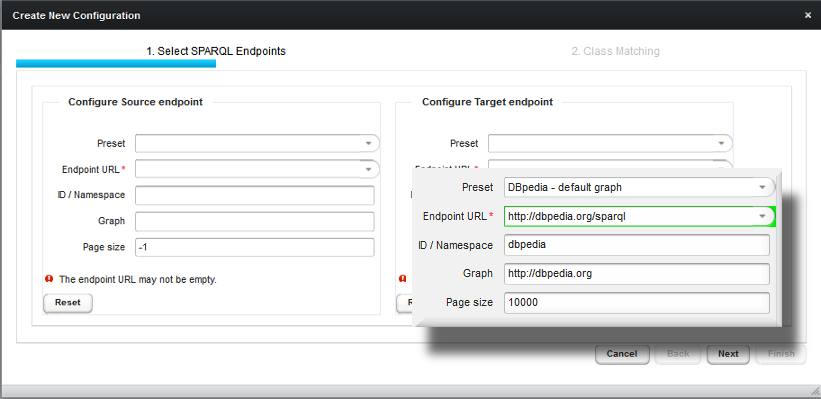
\includegraphics[width=0.95\textwidth]{images/endpoint.png}
		\caption{The Panel to specify the SPARQL endpoints. The front layer shows an example configuration to use DBPedia as an endpoint.}
		\label{fig:endpoint}
	\end{figure}
If a public accessible SPARQL endpoint is used instead, SAIM tests its availability by issueing a simple SPARQL query. If the test for reachability is successful SAIM indicates it by a green margin arround the \texttt{Endpoint URL} field as indicated in the top layer of figure \ref{fig:endpoint}.

If both source and target knowledge bases are specified we confirm it by clicking the \texttt{Next} button. The step is the class setting.

 Note, that we will use the Person11 and Person12 datasets of the Person1 OAEI2010 Benchmark as source and target endpoints throughout this manual.
	\section{Class restriction}
	\label{classes}
	Goal here is to specify the \texttt{rdf:type} of the instances we want to match. Figure \ref{fig:class} shows the Class Matching Step. 
	\begin{figure}[!h]
		\centering
		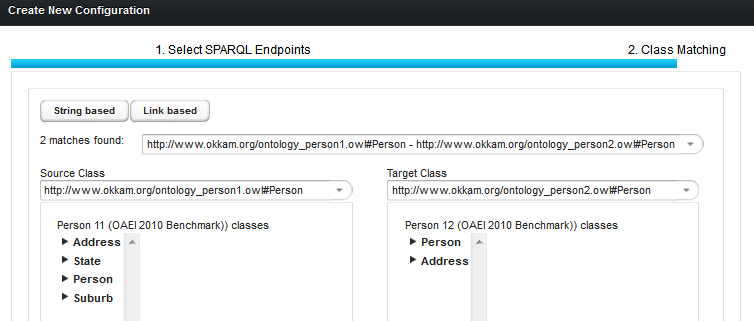
\includegraphics[width=0.95\textwidth]{images/class.png}
		\caption{Class Matching step. Goal is to specify the \texttt{rdf:type} restrictions both source and target instances have to fulfill. The user can manually navigate through the available classes via the class trees or use calculated class matches via	the list at the top. The two buttons \texttt{String based} and \texttt{Link based} at the top will start a new automatic matching process.}
		\label{fig:class}
	\end{figure}
	
	Per default a simple string based comparison off all available classes is computed. Upon finish the user can choose a match in the list at the top of the class matching window. The more sophisticated but time consuming link based comparison could be started manually. This method tries to link \texttt{rdf:type}s via availlable \texttt{owl:sameAs} statements.\todo{More details}. If large knowledge bases such as DBPedia are used to query all availlable classes may take some time, so please stay patient. Once this is done, the user can also navigate through the class and subclass hierachy of an endpoint via the tree at the bottom.
	
	Once two instance types are selected the next and final step of the endpoint specification is to choose the properties the Link Specifications can rely on.
	\section{Property Matching}
	\label{properties}
	Goal of this step is to specify sets of properties for the source and target instances. Note, that the use specifies property matches. These matches will later have an influence on Link Specification learning algorithms based on Genetic Programming. These algorithms will only consider comparisons between these links. So if you're uncertain about corresponding properties we encourage you to choose all possible property pairs. However, the property matching will only restrict learning methods. The user will be free to later manually compare any source property with any target propertiy.
	
	Once again this step is assisted by automatic computed property matches. On default a string based comparison of the property names is computed. But the user can also start a more sophisticated yet complex matching algorithm at the top of the property matching panel. Once all property pairs were defined, we submit the settings by clicking the \texttt{Finish} button. We will return to the main page of SAIM. As
	
 \begin{figure}[!h]
		\centering
		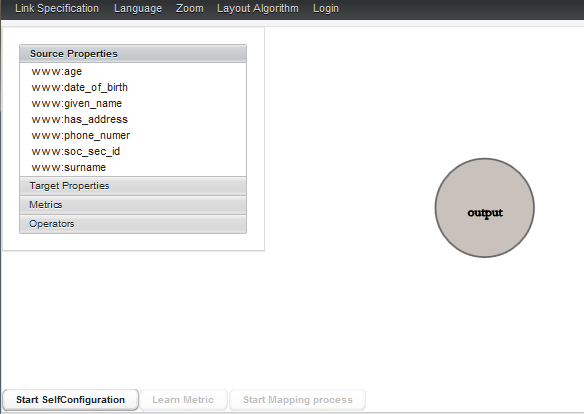
\includegraphics[width=0.95\textwidth]{images/metric_empty.png}
		\caption{The main window of SAIM after specifying the endpoints. The accordion lists of source and target properties on the left hand are filled according to the propties the user selected in the Property Matching step described in section \ref{properties}. This sceenshot is based on the running example Person1 dataset of OAEI2010, depicted in appendix \ref{person1Spec}}
		\label{fig:metric_start}
	\end{figure}
	
%%%%%%%%%%%%%%%%                              MANUAL LINK SPECS 											%%%%%%%%%%%%%%%%%%%%%%%%%
\chapter{Manual metric definition and execution}
\label{manual}
The main window of SAIM enables the user to manually specify a Link Specification without knowing the LIMES grammar in detail. For a formal specification please refer to \cite{NGLY12}.

A Link Specification relies on a specification of \emph{atomic similarity measures} and \emph{similarity measures}. Generally, a similarity measure $m$ is a function such that $m: S \times T \rightarrow [0, 1]$, where $S$ (source) and $T$ (target) are set of enteties. We call a measure atomic when it relies on exactly one similarity measure $\sigma$ (e.g., trigrams similarity for strings) to compute the similarity of a pair $(s, t) \in S \times T$.
We call a link specification atomic if it compares the value of a measure $m$ with a threshold $\theta$, thus returning the pairs $(s, t)$ that satisfy the condition $\sigma(s, t) \geq \theta$.\\  
A link specification $spec(m, \theta)$ is either an atomic link specification or the combination of two link specifications via specification operators such as \texttt{AND} (intersection of the set of results of two specs), \texttt{OR} (union of the result sets), \texttt{XOR} (symmetric set difference), or \texttt{DIFF} (set difference).

\subsection{Measures and Operators}
SAIM supports the following atomic similarity measures two compare the values of two properties: 

\begin{itemize}
	\item \texttt{Cosine} A Vector based String Similarity.
	\item \texttt{Trigrams} The Dice Coefficient based on common trigrams.
	\item \texttt{Levensthein} aka Edit distance.
	\item \texttt{Jaccard} A Token-based coefficient defined as the size of the intersection divided by the size of the union.
	\item \texttt{Overlap}
	\item \texttt{Euclidean} The euclidean distance of two numbers.
\end{itemize}

 To build complex Link Specifications SAIM supports complex measures:

\begin{itemize}
	\item \texttt{MIN}$(m_1, m_2)$ Metric operator, combines the matches of $m_1$ and $m_2$ based on the minimum similarity.
	\item \texttt{MAX}$(m_1, m_2)$ Metric operator, combines the matches of $m_1$ and $m_2$ 
	\item \texttt{ADD}$(m_1, m_2)$ A linear combination, based on coefficients.
	\item \texttt{MULT}$(m_1, m_2)$ A linear combination, based on coefficients.
	\item \texttt{AND}$(m_1, m_2)$ Intersection of the set of results of two specs (based on (local) thresholds).
	\item \texttt{OR}$(m_1, m_2)$ Union of the set of results of two specs (based on (local) thresholds).
	\item \texttt{XOR}$(m_1, m_2)$ Symmetric set difference of the set of results of two specs (based on (local) thresholds).
	\item \texttt{DIFF}$(m_1, m_2)$ Set difference of the set of results of two specs (based on (local) thresholds).
\end{itemize}

\subsection{Buildung a Link Specification}
Figure \ref{fig:metrics} shows an example of an atomic and a complex Link Specification.
\begin{figure}
        \centering
        \begin{subfigure}[b]{0.30\textwidth}
                \centering
								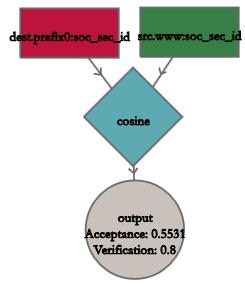
\includegraphics[width=\textwidth]{images/atomic1.png}
                \caption{Atomic Link Specification}
                \label{fig:atomic}
        \end{subfigure}
				\hspace{0.3cm}
				\begin{subfigure}[b]{0.6\textwidth}
                \centering
								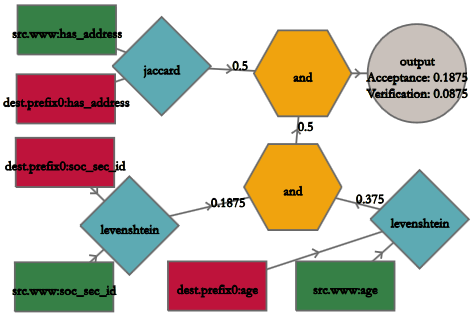
\includegraphics[width=\textwidth]{images/complex1.png}
                \caption{Complex Link Specification}
                \label{fig:complex}
        \end{subfigure}
        \caption{Examples of Link Specifications. Basesd upon example \ref{person1Spec}.}
\label{fig:metrics}
\end{figure}

In order to build a atomic Link Specification as depicted in \ref{fig:simple} the user has to do:

\begin{enumerate}
	\item Choose a source property from the accordion panel (e.g. \texttt{www:soc\_sec\_id} as in \ref{fig:atomic})
	\item Choose a target property from the accordion panel (e.g. \texttt{pefix0:soc\_sec\_id} as in \ref{fig:atomic})
	\item Choose a atomic similarity measure from the accordion panel (e.g. \texttt{cosine} as in \ref{fig:atomic})
	\item Connect both properties with the measure (right-click on the property, choose \textit{Link to} from the context menu, left-click on the measure)
	\item Connect the measure with the output node (right-click on the measure, choose \textit{Link to} from the context menu, left-clcik on the Output node).
	\item Double-click the Output node and set/adjust the thresholds.
\end{enumerate}

Note that several nodes in the Link Specification tree have parameters to be set. To do so \textbf{double-click} the node.
\begin{itemize}
	\item Property nodes: Select preprocessing functions for property.
	\item Operator nodes: Set parameters: local thresholds/coefficients for child specs.
	\item Output Node: global acceptance(verification) threshold.
\end{itemize}

\subsection{Executing a Link Specification}
To run a Link Specification click the button \texttt{Start Mapping process}. First the specified metric is checked if it is complete and valid. If everything is ok, the mapping process is started and a new window shows the progress. The results will be presented in the Mapping Window as depicted in figure \ref{fig:execution}.\\
 The \textbf{table} at the bottom shows instance pairs of the specified source and target endpoint which fulfill the Link Specification. Clicking on a row will present the fetched data of botch matched instances above the table. Clicking on a link will try to dereferentiate the corresponding instance by its URI in a separat browser tab. The \texttt{value} column holds the similarity value of the matches.\\To \textbf{download} the complete mapping click the \texttt{Save} button beneath the table. This will open a sub window, to choose different serialization format. As of now, we support Turte, N-Triple and Tab-seperated files.
 
 \begin{figure}[!h]
		\centering
		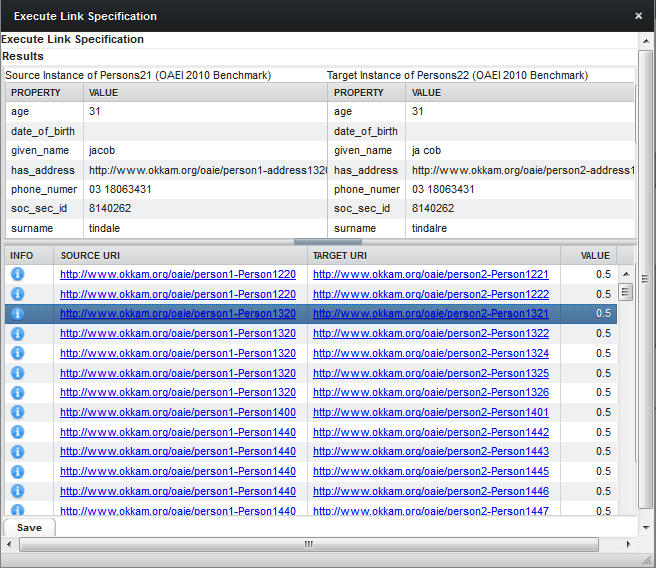
\includegraphics[width=0.95\textwidth]{images/execution_window.png}
		\caption{Mapping window presents results (Mapping) of a Link Specification. This are the results of executing the Link Specification of \ref{complex}.}
		\label{fig:execution}
	\end{figure}

%%%%%%%%%%%%%%%%%                             SELFCONFIGURATION 											%%%%%%%%%%%%%%%%%%%%%%%%%
\chapter{Selfconfiguration}
\label{selfconfig}
SAIM also supports unsupervised machine learning method of Link Specifications, called \emph{Selfconfiguration}. Once all endpoints are specified as described in chapter \ref{kbdefinition} this option is available. These machine learning methods rely on so-called Psuedo F-Measures. \todo{cite EUCLID paper}.\\
To start click the \texttt{Start Selfconfiguration} on the main window of SAIM.
\subsection{Mesh based Selfconfiguration}
There are several deterministic selfconfiguration algorithms available trying to discover high quality Link Specifications baes upon different classifier. Other parameters to adjust are:

\begin{itemize}
	\item Beta $\beta \in [0,1]$ value of the Pseudo F-measure.
	\item Number of iterations to learn.
	\item Minimal coverage over all instances for a property.
\end{itemize}

\subsection{Selfconfiguration based on Genetic programming}
Besides the parameters described above the user can set additional parameters for the Genetic Programming approach. These are:
\begin{itemize}
	\item Number of generations to evolve
	\item Number of individuals in a population
	\item Corssover and mutation probality
\end{itemize}
Whereas, the first two influence the runtime of the algorithm.

%%%%%%%%%%%%%%%%%                                  LEARNING 													%%%%%%%%%%%%%%%%%%%%%%%%%
\chapter{Improving results through learning}
\label{learning}
SAIM also implements supervised learning algorithms presented in \cite{NGLY12}. If all endpoints are specified as described in chapter \ref{kbdefinition} and an intial Lnk Specification has been set either manually or through self configuartion as decribed in chapter \ref{manual} and \ref{selfconfig} respectively. The initial Link Specification is required to retrieve initial training data to be annoted by the user.\\
All learning algorithms are based on Genetic Programming. Beside the typical parameters like Population size and number of generations to evolve and mutation propability the user can set the \texttt{number of inquiries} presented each iteration. To start the learning process the user can choose between active and batch learning approaches. In order to get good results we recommend a higher number of inquiries. There are 3 active learning approaches implemented. The basic EAGLE active learning approach \cite{NGLY12} and two enhancements using correlation features to better estimate the quality of examples to be classified. One is based on clustering the other uses a graph based features of spreading activation \cite{NGO+13}.\\
Either way, the user evaluates the examples through checkboxes added to a equivalent table representation of the possible links as depicted in figure \ref{fig:execution}. Again, the number of generations to evolve and the population size have the most influence at runtimes.
%%%%%%%%%%%%%%%%%                                  FEATURES 													%%%%%%%%%%%%%%%%%%%%%%%%%
\chapter{Additional features}
\label{features}

\section{Caching}
\label{caching}


\section{Import and save Link Specifications}
\label{ImportExport}

\section{Uploading RDF dumps}
\label{upload}

\bibliographystyle{plain}
\bibliography{saim}

\newpage
\appendix
\chapter{}
\section{The menu bar}
\label{menuBar}


\section{Person1 Running example: sample Configuration}
\label{person1Spec}
This is a sample configuartion we use as a running example throughout this manual. We link the Person11 and Person12 dataset of the Persons1 OEI2010 Benchmark.\\
\lstset{language=XML}
\lstinputlisting[language=XML, firstline=0, lastline=61]{linkspec.xml}

\end{document}